\subsection{Pager e Criteria API}

La classe che si occupa del recupero delle informazioni dal database è \texttt{ContractSearchService}. Lo scopo di questa classe è effettuare un ricerca paginata sul database secondo vari criteri di ricerca quali 
responsabile scientifico, data, dittà etc. Il codice che si occupa della paginazione è stato incapsulato nella classe \texttt{ResultPager}. \texttt{ResultPager} viene costruito
col metodo:

\begin{lstlisting}
&&ResultPagerBean(int currentPage, int pageSize, TypedQuery<T> query,
&&			TypedQuery<Long> countQuery) 
\end{lstlisting}

Come si può vedere è possibile impostare il numero di risultati per ogni pagina, la pagina corrente e naturalmente la query che vogliamo eseguire. Per ottenere una pagina di risultati è sufficiente chiamare \lstinline{getCurrentResults()}
mentre è possibile spostarsi da una pagina all'altra tramite \lstinline{next()} e \lstinline{previous()}

\texttt{ContractSearchService} viene specializzato, per poter eseguire la paginazione, tramite la composizione con un oggetto di tipo \texttt{Pager}, l'interfaccia che \texttt{ContractSearchService} e \texttt{ResultPager} implementano, come
illustrato in figura \ref{pager}


\begin{figure}[h]
  \caption{Digramma delle classi per Pager}
  \label{pager}
  \centering
    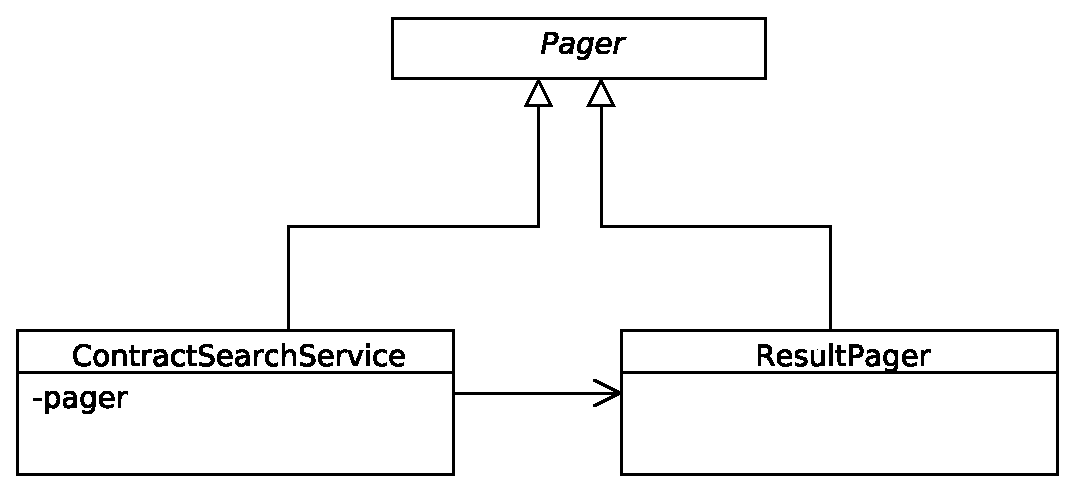
\includegraphics[width=0.7\textwidth]{pager.eps}
\end{figure}

